\documentclass[letterpaper]{article} % Feel free to change this

\usepackage{graphicx}
\usepackage[english]{babel}
\usepackage[utf8]{inputenc}
\usepackage{fancyhdr}
 
\pagestyle{fancy}
\fancyhf{}
\rhead{Week of Jan 21}
\lhead{CS 270 Helper Material}

\setlength\parindent{0pt}


\begin{document}

\section{State Space}

\subsection{Counting State Space}

If you have $N$ nodes in a graph, and you are representing your state based only on where you are, how many different states are there?\\

\noindent
Answer: $N$\\

\noindent
What about if you are representing states as only visited or not visited. Now how many states are there?\\

\noindent
Answer: $2^N$\\

\noindent
Lastly, what about if you combine the two and represent state based on where you are and what you have visited?\\

\noindent
Answer: $N2^{N - 1}$  because including where you currently are in visited is redundant. $N2^{N}$ would also be acceptable if this optimization is note made. $N$ tracks where you currently are, and $2^{O(n)}$ tracks where you have visited.\\

\noindent
How does it change if track the number of visits to each node and the number of visits is bounded to $M - 1$?\\

\noindent
Answer: $NM^{N - 1}$  because including where you currently are in visited is redundant. $NM^{N}$ would also be acceptable if this optimization is note made as before. Now, each visited entry has $M$ possible values, $0$ to $M - 1$, rather than just 2.

\subsection{Successor Function}

Talk about what the abstraction of a successor function is.\\

\noindent
If $S$ is your state, $S'$ is the set of possible next states, and $F$ is your successor function, then:\\

$$S' = F(S)$$

\noindent
Why is this a useful abstraction for programming? Allows us to abstract the derivation of next states from our current state, and we can reuse serach algorithms by just providing new successor functions. And so on.

\section{Search Algorithms}

\subsection{Terminology}

\begin{itemize}
	\item Fringe - set of nodes generated, but not expanded
	\item Goal Function - checks if a node is the goal
	\item Successor Function - defines possible next states from current state (see above section)
\end{itemize}

\noindent
Using this, we can define a generic search function as:\\

\noindent
Initialize the fringe with the start state. While the fringe isn't empty, pick a state off of the fringe. Use the goal function to check if the state is a goal. If it is then you are done: SUCCESS. If not, then use the successor function to generate all next states $S'$, and add those to the fringe. Repeat until success or the fringe is empty, FAIL.

\subsection{BFS}

Explain what breadth first search is, and how it uses a first in first out data structure. \textbf{**Draw tree search examples**}.\\

\textbf{Properties:}

\begin{itemize}
	\item Complete: if there is a solution, BFS will find it
	\item Finds the shallowest solution in the tree (not always the lowest cost with non uniform edge weights)
\end{itemize}

\textbf{Runtime}\\

With branching factor $b$ (maximum number of successors), and a max depth $d$, runtime and space are $O(b^d)$.

\subsection{DFS}

Explain what DFS is and how it uses a last in first out data structure. \textbf{**Draw tree search examples**}.\\

\textbf{Properties:}

\begin{itemize}
	\item Not complete: could get caught in cycles and never escape
	\item No guarantees about what depth a solution will be found at
\end{itemize}

With branching factor $b$ (maximum number of successors), and a depth $d$, runtime is unbounded due to lack of completeness and space is $O(bd)$. With no cycles or visited state detection to prevent visiting cycles, runtime is $O(b^d)$.

\subsection{Depth Limited DFS}

Just like DFS, except never go deeper than some depth $d$. Keeping track of current depth is very easy.

\subsection{Iterative Deepening}

Run depth limited dfs for $n=1$, then depth limited dfs $n=2$, then depth limited dfs $n=3$, and so on until a solution is found.\\

Uses the same space requirements as dfs. Really not as wasteful as it seems because almost all work is done at the last level of the tree.

\section{Nonuniform Edge Weights}

\subsection{Uniform Cost Search}

Idea is as follows, always work on the lowest cost node. he cost of a node is defined as the total cost to get to that node, not the cost of the edge leading up to it. BFS is an implementation of this for uniform cost edges. Uniform cost search is equivalent to Dijkstras without visited state detection.

\subsection{Searching Backwards From Goal}

Sometimes, working backwards from the solution is an effective way to find the path to the solution. One such application is bidirectional search. Then the runtime goes from $O(b^{d})$ to $O(b^{\frac{d}{2}})$.

\section{Heuristic Searches}

\subsection{Heuristic}

A heuristic function $h(n)$ gives an estimate of the instance from $n$ to the goal. $h(goal) = 0$. 

\subsection{Greedy Best First Search}

Greedy best first search always expands the node with the lowest $h$ value in the fringe.\\

It would be good to draw an example up on the board here. Draw a graph $G = (E,V)$, give all edge weights, a start, a goal, and $h(n)$ for all $n \in V$.

\subsection{A* Search}

Takes into account both the cost accrued so far as well as the expected cost to goal (heuristic). Let $g(n)$ be the cost already incurred along path $n$. Expand nodes with lowest $g(n) + h(n)$.\\

If your heuristic is bad, this may not give you the optimal solution. If $h(n) = 0$ for all $n \in V$, then this is uniform cost search, which we know is optimal.\\

A heuristic is said to be \textbf{admissible} if it never overestimates the distance to the goal. It is either equal to or less than the actual cost to goal. Formally, if $n$ is the optimal solution reachable from $n'$, then 

$$g(n) \geq g(n') + h(n')$$

It can be proven that if the heuristic is admissible, then A* will return an optimal solution. Please see proof in slides if you would like to derive in helper hours.

\begin{figure}[h]
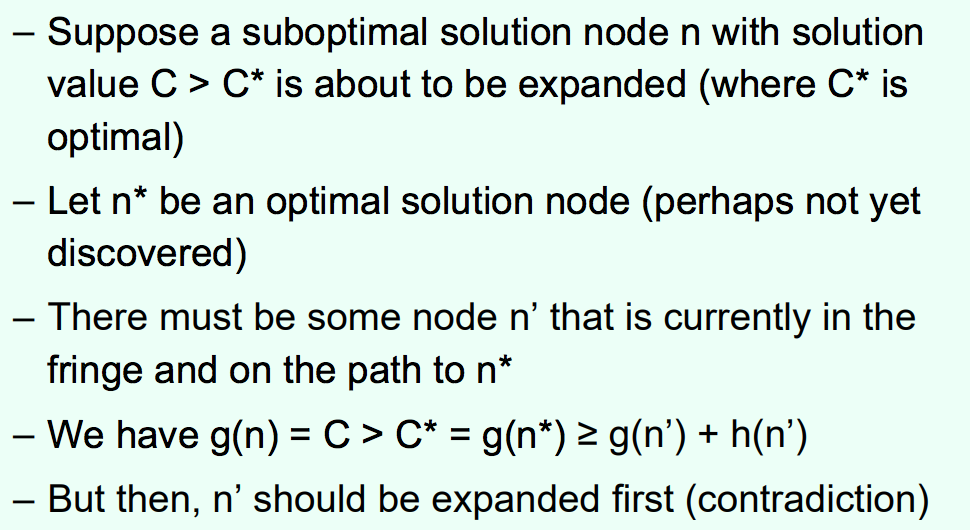
\includegraphics[width=8cm]{proof.png}
\centering
\end{figure}

\end{document}
